\documentclass[runningheads]{llncs}

\usepackage{graphicx}
\usepackage{amsmath,amssymb,amsfonts}
\usepackage{booktabs}
\usepackage{array}
\usepackage{microtype}
\usepackage{algorithm}
\usepackage{algpseudocode}
\usepackage{url}

% llncs does not define a proof environment; define a minimal one (guarded so it is
% only added if not already present, e.g. if amsthm is loaded later).
\makeatletter
\@ifundefined{proof}{%
  \newenvironment{proof}[1][Proof]{\par\noindent\textbf{##1.}\hspace*{1em}\ignorespaces}{\hfill\ensuremath{\square}\par\medskip}%
}{}
\makeatother

\begin{document}

\title{Beyond Feasibility: Multi-Objective Constraint Optimization for Automated Examination Paper Generation}

\titlerunning{Beyond Feasibility in Automated Exam Generation}

% Anonymized for ICAA double-blind review
\author{Anonymous Author(s)}
\authorrunning{Anon. Author(s)}
\institute{Institute Anonymized for Double-Blind Review\\
\email{author@domain.org}}

\maketitle

\begin{abstract}
Automated examination paper generation in large-scale assessment platforms can be formulated as a Boolean Constraint Satisfaction Problem (CSP) under structural, temporal, topic-coverage, and non-duplication constraints.
A first-feasible solver can generate a structurally valid paper efficiently, but it treats all feasible papers as equivalent and therefore provides no guarantee of alignment with a desired difficulty distribution or examination blueprint.
We present a reproducible policy formulation for a deployed commercial examination platform: a lexicographic CP-SAT configuration that prioritizes difficulty-distribution alignment, then topic coverage, and finally soft blueprint-compliance goals---instantiated in our study as Bloom's-taxonomy fit---while enforcing non-negotiable blueprint rules as hard constraints.
We evaluate this as a single-corpus systems case study on 475 CBSE Class X Mathematics items, with calibrated synthetic pools used only for solver scaling to $N{=}10{,}000$.
The evaluation measures structural blueprint quality, feasibility behaviour, and solver runtime (excluding embedding and conflict-graph construction);
it does not establish psychometric validity or end-to-end latency. The shared suite compares five policies ($B0$, $B_G$, $B1$, $B2$, $B3$);
$B0$-R is a separate ordering-sensitivity diagnostic. Of 80 deterministic shared blueprints, 70 are feasible for all five policies;
in the other 10, every sequential policy reaches a CP-SAT-certified infeasible later-section continuation (with no timeouts, UNKNOWN outcomes, or skips), which does not by itself certify global blueprint infeasibility.
On the 70 common cases, median $(D,\mathrm{Bloom},\mathrm{solver\ runtime\ per\ complete\ paper})$ is $(52,40,0.03\,\mathrm{s})$ for B0, $(40,24,0.13\,\mathrm{s})$ for B1, and $(40,22,0.07\,\mathrm{s})$ for default weighted B2.
Thus the contribution is policy interpretability and reproducible engineering, not a claim of uniform optimization dominance: B1 makes a deterministic, weight-free priority order explicit, whereas B2 has the strongest aggregate quality--solver-runtime trade-off observed in this corpus.
\keywords{Constraint Satisfaction Problem \and Multi-Objective Optimization \and Automated Test Assembly \and CP-SAT \and Lexicographic Optimization \and Near-Duplicate Detection \and Educational Assessment.}
\end{abstract}

%===============================================================================
\section{Introduction}
\label{sec:intro}
%===============================================================================

Large-scale educational assessment platforms manage repositories containing tens of thousands of test items.
Assembling an examination paper from these banks is far more complex than executing a database retrieval query.
Each paper must satisfy a stringent combination of structural, temporal, pedagogical, and blueprint constraints specified by examination boards (e.g., CBSE, ICSE): exact total marks, strict duration limits, section-wise question counts, balance across cognitive levels (Bloom's taxonomy~\cite{bloom1956,anderson2001}), topic coverage, and the strict avoidance of duplicate or near-duplicate questions.
National policy frameworks such as India's National Education Policy~\cite{moenep2020} further emphasise competency-based assessment, making blueprint compliance a first-class engineering requirement rather than an aesthetic preference.

\subsection{The Feasibility Gap and a Running Example}
Most production systems treat generation as a Constraint Satisfaction Problem (CSP) and employ SAT or CP solvers configured to terminate at the \emph{first feasible solution} ($B0$).
While computationally efficient, first-feasible solving exhibits a major flaw: \textbf{a feasible paper is not necessarily a high-quality paper}.

\begin{table}[t]
\caption{Running example: toy 3-band illustrative example ($N{=}8$) demonstrating the feasibility gap. The production empirical model uses 7 ordinal difficulty bands.
Target specification: $M{=}10$ marks, $K{=}4$ questions, target difficulty histogram $\Delta=(2\text{ Easy},2\text{ Medium},0\text{ Hard})$.}
\label{tab:running_example}
\centering
\small
\begin{tabular}{ccccccc}
\toprule
\textbf{Item} & \textbf{Marks} $m_i$ & \textbf{Difficulty} $d_i$ & \textbf{Topic} $T_i$ & $B0$ & $B1$ \\
\midrule
$q_1$ & 2 & Easy   & Algebra       & \checkmark & \checkmark \\
$q_2$ & 2 & Easy   & Geometry      & \checkmark & \checkmark \\
$q_3$ & 3 & Easy   & Trigonometry  & \checkmark & -- \\
$q_4$ & 3 & Easy   & Algebra       & \checkmark & -- \\
$q_5$ & 3 & Medium & Geometry      & -- & \checkmark \\
$q_6$ & 3 & Medium & Trigonometry  & -- & \checkmark \\
$q_7$ & 5 & Hard   & Algebra       & -- & -- \\
$q_8$ & 5 & Hard   & Calculus      & -- & -- \\
\bottomrule
\end{tabular}
\end{table}

Consider the toy bank in Table~\ref{tab:running_example}.
Both candidate papers satisfy the hard constraints ($M{=}10$, $K{=}4$). However, the baseline $B0$ halts at the first feasible solution it encounters and returns a paper consisting entirely of Easy questions, giving difficulty deviation $D(B0)=|4{-}2|+|0{-}2|+|0{-}0|=4$ versus the target $\Delta$.
An optimized solver ($B1$) instead selects $\{q_1,q_2,q_5,q_6\}$, attaining $D(B1)=0$ (a perfect difficulty match) while also maximizing topic coverage across Algebra, Geometry, and Trigonometry.
The gap between $D(B0)=4$ and $D(B1)=0$ is the \emph{feasibility gap} this paper attacks.
(For illustration we use a 3-band simplification; the production bank uses seven difficulty bands.)

\subsection{Research Questions and Contributions}
This work addresses the problem of transforming a deployed first-feasible engine into a multi-objective optimization platform.
We investigate five research questions:
\begin{itemize}
    \item \textbf{RQ1 (Quality):} How much does lexicographic optimization improve difficulty alignment and topic coverage over first-feasible generation?
    \item \textbf{RQ2 (Solver runtime):} What solver-runtime overhead does optimization introduce as banks scale to $N=10{,}000$, excluding embedding and conflict-graph construction?
    \item \textbf{RQ3 (Blueprint tightness):} How does the optimization gain behave as the feasible region contracts?
    \item \textbf{RQ4 (Duplicate detection):} How does an entity-gated SBERT detector behave on a constructed, corpus-specific near-duplicate stress test?
    \item \textbf{RQ5 (Compliance):} To what extent does explicit optimization of soft blueprint requirements improve structural blueprint compliance over first-feasible generation?
\end{itemize}

\noindent\textbf{Pipeline boundary for duplicate detection.} Duplicate detection is deliberately treated as a pre-solver graph-filtering stage rather than as a competing optimization objective: the semantic detector constructs the conflict graph $S$, and CP-SAT consumes $S$ as a hard at-most-one constraint.
RQ4 therefore characterizes a boundary condition of the overall pipeline---specifically, whether entity density in this STEM corpus limits the ability of the gate to filter semantic false positives---rather than claiming a separate contribution in semantic duplicate detection.

\noindent\textbf{Contributions.} (1) A formal selection-CSP model derived from a deployed examination-generation system;
(2) a reproducible, deterministic three-pass CP-SAT policy formulation that sequentially optimizes difficulty alignment, topic coverage, and soft blueprint compliance while preserving hard constraints;
(3) a formal blueprint-compliance framework separating non-negotiable structural rules from graded distributional goals;
(4) a controlled comparison of first-feasible, greedy, lexicographic, weighted, and soft-window policies;
and (5) an executable evidence package for a 475-item single-corpus systems case study and calibrated solver-scaling experiments.
The contribution is policy interpretability and reproducible engineering in this setting, not a claim of universal optimization dominance.

%===============================================================================
\section{Related Work}
\label{sec:related}
%===============================================================================

\subsection{Automated Test Assembly}
Automated Test Assembly (ATA) is a mature subfield of psychometrics and operations research.
The foundational formulation due to Theunissen~\cite{theunissen1985} and the IRT-based LP/MILP models of van der Linden and colleagues~\cite{vanderLinden2005,vanderLinden1989,lord1980} cast paper construction as 0--1 integer programming, selecting items to maximize a target information function subject to content and length constraints.
These approaches are powerful but assume \emph{calibrated IRT item parameters} (discrimination, difficulty, guessing) estimated from large student-response datasets.
Non-IRT lines---greedy and dynamic-programming test-sheet composition for large banks~\cite{hwang2006} and modern adaptive assembly~\cite{vanderLinden2010}---likewise presuppose calibrated statistics.
Such parameters are rarely available in K--12 publishing or coaching-institute settings, where items carry only coarse metadata (marks, time, an ordinal difficulty, topic and cognitive-level tags).
Our model therefore targets the data regime ATA explicitly assumes away.
The contribution is not a new general-purpose ATA algorithm: it is a deployable CP-SAT formulation, explicit policy comparison, and reproducibility package for this metadata-only setting.

\subsection{Constraint Programming and CP-SAT}
Constraint programming and SAT-based solvers have become strong alternatives for discrete selection, with lazy-clause-generation~\cite{nieuwenhuis2006} and modern CDCL SAT engines~\cite{biere2009} underpinning tools such as Google OR-Tools CP-SAT~\cite{ortools,perron2023}.
CP-SAT is well-suited to our setting because it natively expresses Boolean decision variables, linear equalities, and---crucially---pairwise at-most-one constraints that arise from duplicate conflicts, while providing bounded-optimal search with controllable time budgets.

\subsection{Semantic Near-Duplicate Detection}
Transformer-based sentence embeddings, notably Sentence-BERT~\cite{reimers2019} (built on BERT~\cite{devlin2019}), are widely used for semantic similarity and deduplication, with dedicated similarity benchmarks~\cite{agirre2012};
classic lexical methods such as SimHash~\cite{charikar2002} remain relevant for scale.
In STEM banks, embedding similarity alone can over-flag \emph{structural} variants (e.g., ``Is $4$ even?'' vs.\ ``Is $6$ even?'') that share boilerplate but differ in the mathematical entities under test.
Our deployed hybrid detector gates embedding similarity with a spaCy~\cite{spacy2020} entity-overlap check designed to test this mitigation.
The resulting conflict graph $S$ is a pipeline boundary: it is constructed before CP-SAT and contributes the at-most-one constraints in \eqref{eq:conflict}.
RQ4 therefore characterizes how entity density limits this semantic pre-filter in the present STEM corpus;
it does not establish improvement over pure vector similarity.

\subsection{Educational Blueprints and Compliance}
Cognitive taxonomies~\cite{bloom1956,anderson2001}, validity standards for educational testing~\cite{standards2014}, and policy mandates for competency-based assessment~\cite{moenep2020} codify what a ``valid'' paper must look like: prescribed difficulty mixes, coverage of all syllabus units, and spreads across cognitive levels.
Systematic reviews of automated and educational question handling~\cite{kurdi2020} note that compliance is typically enforced informally.
We instead formalize blueprint compliance as a constraint family with hard and soft components and a reproducible graded score.

\subsection{Positioning}
Table~\ref{tab:positioning} contrasts this work with the streams above across six dimensions.
The novelty is in this domain-specific formulation and evidence package, rather than in claiming a new generic optimization primitive.

\begin{table}[t]
\caption{Positioning of this work relative to existing research streams.}
\label{tab:positioning}
\centering
\scriptsize
\begin{tabular}{lcccc}
\toprule
\textbf{Dimension} & \textbf{Traditional ATA} & \textbf{Standard CSP/ILP} & \textbf{NLP Dedup} & \textbf{This Work} \\
\midrule
Primary focus & Psychometric IRT & Feasibility & Text similarity & Quality \& compliance \\
Solver paradigm & MILP / LP-relax. & Single-pass CSP & N/A & Three-pass CP-SAT with lexicographic objectives \\
Duplicate handling & Manual exclusions & Basic ID check & Vector cosine & Hybrid SBERT + entity gate \\
Board compliance & Informal rules & Hard rules only & N/A & Hard + soft formalization \\
Objective model & Single target info & Feasible / single-obj & N/A & Lexicographic multi-obj \\
Problem source & Theoretical / small & Synthetic banks & Text corpora & Deployed commercial system \\
\bottomrule
\end{tabular}
\end{table}

%===============================================================================
\section{Problem Formalization}
\label{sec:formalization}
%===============================================================================

Let $Q=\{q_1,\dots,q_n\}$ be an item bank of $n$ questions.
Each item $q_i=(m_i,t_i,T_i,d_i,\tau_i)$, where $m_i\in\mathbb{Z}^+$ is the marks allocation, $t_i\in\mathbb{Z}^+$ is the estimated completion time (minutes), $T_i\subseteq\mathcal{T}$ is the set of topic/subtopic tags, $d_i\in\{1,\dots,|D|\}$ is an ordinal difficulty band, and $\tau_i$ is the textual content.
We distinguish an \emph{eligibility set} $E\subseteq\mathcal{T}$, which determines which tagged items may be selected, from a \emph{required-coverage set} $R\subseteq\mathcal{T}$, whose topics should be represented in the generated paper.
A blueprint is therefore $B=(M,W,K,E,R,\Delta,\mathcal{H},\mathcal{S})$, where $M$ is total marks, $W$ duration, $K$ question count, $\Delta=(\Delta_1,\dots,\Delta_{|D|})$ is the target difficulty histogram with $\sum_k\Delta_k=K$, and $\mathcal{H}$ and $\mathcal{S}$ denote hard and soft blueprint requirements.

\subsection{Decision Variables and Baseline $B0$}
We introduce a binary decision variable $x_i\in\{0,1\}$ per item ($x_i=1$ iff $q_i$ is selected).
The deployed baseline feasibility problem ($B0$) seeks $x\in\{0,1\}^n$ satisfying:

\begin{align}
\sum_{i=1}^n m_i x_i &= M \quad &&\text{(Exact total marks)} \label{eq:marks} \\
\sum_{i=1}^n t_i x_i &= W \quad &&\text{(Exact total duration)} \label{eq:time} \\
\sum_{i=1}^n x_i &= K \quad &&\text{(Exact question count)} \label{eq:count} \\
x_i + x_j &\le 1 \quad \forall (i,j)\in S \quad &&\text{(Anti-duplicate)} \label{eq:conflict} \\
x_i = 1 &\Rightarrow T_i\cap E\neq\emptyset \quad \forall i \quad &&\text{(Topic eligibility)} \label{eq:eligibility}
\end{align}

\noindent where $S\subseteq Q\times Q$ is the set of near-duplicate pairs (\S\ref{sec:baseline}).
Constraints~\eqref{eq:marks}--\eqref{eq:count} are linear \emph{equalities}; \eqref{eq:eligibility} is a set-membership filter realized by fixing $x_i=0$ for items whose tags are disjoint from $E$; and \eqref{eq:mandatory} explicitly enforces mandatory topic inclusion.
Required topic coverage is a \emph{hard} requirement when the blueprint specifies mandatory topics: for every $t\in R_{\mathrm{hard}}\subseteq R$,
\begin{equation}
\sum_{i:\,t\in T_i}x_i \ge 1 \qquad \forall t\in R_{\mathrm{hard}}.
\label{eq:mandatory}
\end{equation}
Thus mandatory coverage is part of $\mathcal{H}$ and is enforced during every feasibility and optimization pass; it is not merely an eligibility filter. The optional/graded coverage component uses indicators $y_t$ for $t\in R$ and is optimized in Pass~2. The baseline has \textbf{no objective}: any solution satisfying the hard constraints is acceptable, and the solver returns the first one found.

\subsection{Complexity}
\begin{theorem}
Feasibility of the $B0$ baseline CSP is NP-complete.
\end{theorem}
\begin{proof}
We reduce from the \emph{cardinality-constrained subset sum} problem, which is NP-complete~\cite{garey1979}: given positive integers $Z=\{z_1,\dots,z_n\}$, a cardinality $K$, and a target $V$, decide whether some subset of exactly $K$ elements of $Z$ sums to $V$.
Given such an instance, construct an item bank with $m_i=z_i$, $t_i=1$, $S=\emptyset$, and $E=\mathcal{T}$ (all items eligible), and set $M=V$, $W=K$.
Constraint~\eqref{eq:count} forces exactly $K$ selections, so the time equality is automatically satisfied; \eqref{eq:marks} requires $\sum_i z_i x_i=V$.
Hence $B0$ is feasible iff some size-$K$ subset of $Z$ sums to $V$, proving NP-completeness; the multi-objective extension is NP-hard.
\end{proof}

%===============================================================================
\section{Deployed Baseline Architecture}
\label{sec:baseline}
%===============================================================================

The production platform operates the three-tier pipeline of Figure~\ref{fig:architecture}.
Generation is performed \emph{per section} of a paper template, with two accumulators carried across sections---selected IDs and their texts---so that no later section reuses an earlier one's items.

\begin{figure}[t]
\centering
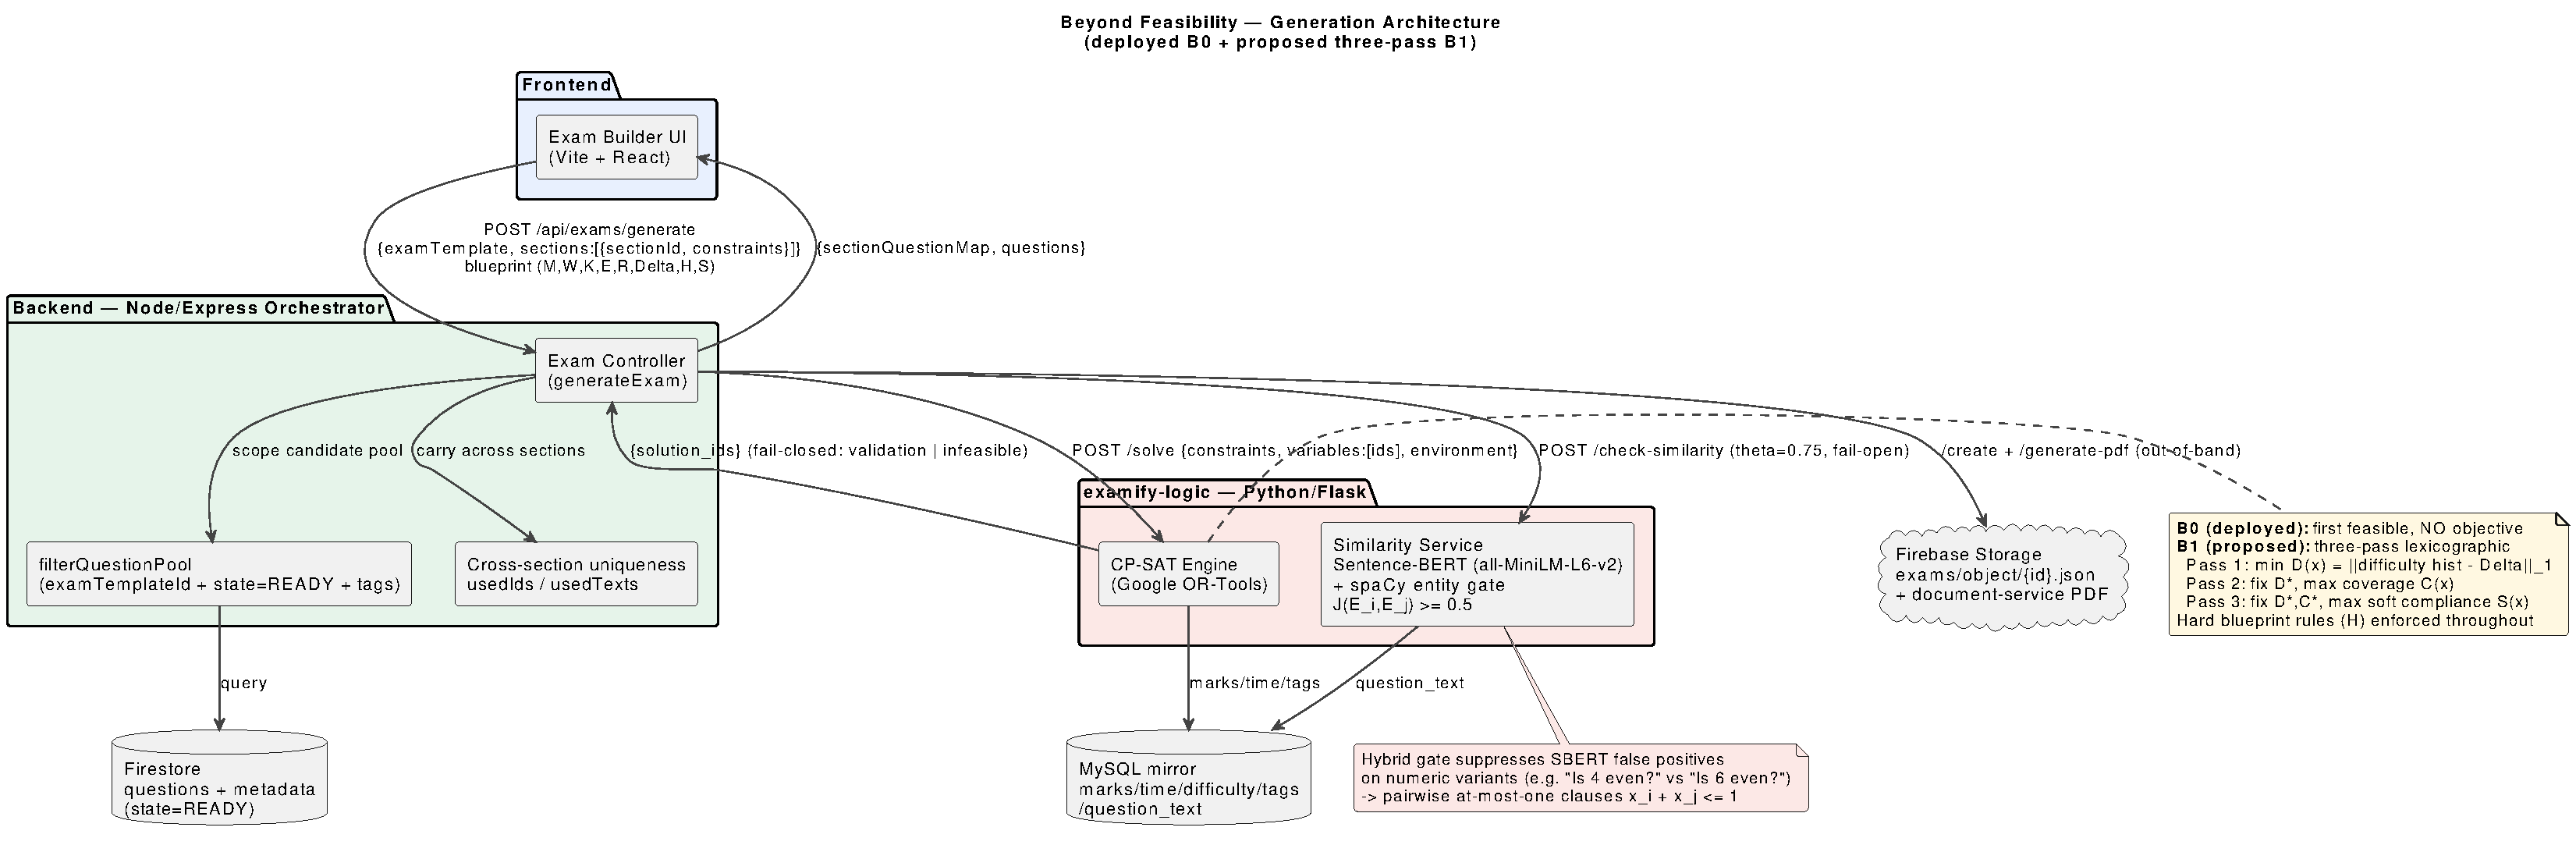
\includegraphics[width=\textwidth]{architecture.pdf}
\caption{Three-tier deployed generation pipeline. The orchestrator loops over template sections, enforcing cross-section uniqueness.}
\label{fig:architecture}
\end{figure}

\begin{enumerate}
    \item \textbf{Metadata pre-filtering.} The orchestrator scopes the repository to a candidate pool $Q$ by template, readiness state, and required tags.
A cheap \emph{necessary-condition} pre-check (cardinality $K\le n$, marks and time within their feasible bounds $M\in[\min_i m_i,\sum_i m_i]$ and $W\in[\min_i t_i,\sum_i t_i]$, sufficient tag-matching items) rejects obviously infeasible blueprints before optimisation begins.
    \item \textbf{Hybrid duplicate detection.} Candidate texts $\tau_i$ are cleaned (stripping \texttt{Q.} prefixes and \LaTeX{} wrappers) and encoded with Sentence-BERT.
A pair with cosine similarity $\ge\theta_s$ passes a mathematical entity/token gate;
if the entity/token Jaccard overlap $J(E_i,E_j)\ge 0.5$, an undirected edge $(i,j)$ is added to $S$.
Here $E_i$ contains extracted numerical tokens, variables, units, named quantities, and other domain-specific entities rather than relying on generic named-entity recognition alone.
The gate suppresses SBERT false positives on templated numeric items.
(In production, the in-solver pairwise gate operates at $\theta_s{=}0.75$ while the HTTP-facing duplicate check uses $0.85$; this threshold drift is documented as a limitation.)
    \item \textbf{CP-SAT engine ($B0$).} Google OR-Tools CP-SAT~\cite{ortools} solves over $x_i$ and constraints~\eqref{eq:marks}--\eqref{eq:eligibility} with a 30\,s budget, returning the first feasible assignment.
The orchestrator \emph{fails closed}: on infeasibility it surfaces a typed diagnostic (validation vs.\ infeasible) rather than silently degrading;
similarity failures, by contrast, fail open.
\end{enumerate}

\noindent\textbf{Sequential assembly and continuation failures.} Production assembly deliberately solves template sections one at a time: each section has its own marks, time, and count limits, while selected IDs and their texts are carried forward to prevent cross-section reuse.
This decoupling reflects the production orchestration boundary: it supports section-level limits and diagnostics and prevents overlap between independently configured template sections.
It also introduces a policy-dependent form of greedy lock-in: an item choice made while solving an earlier section can consume a scarce item or combination of marks/time that a later section needs.
Consequently, a CP-SAT \texttt{INFEASIBLE} status in the RQ1 sequential harness certifies only a \emph{sequential continuation failure} for that policy path---no assignment can extend the already selected earlier sections under the remaining constraints.
It is \emph{not} a certificate that the corresponding whole-paper model, if all sections were solved jointly, has no feasible assignment.
The 10 RQ1 cases reported as infeasible therefore measure failure of the deployed sequential continuation policy, not global blueprint infeasibility.

\noindent\textbf{Honest engineering limitations.} (i) The solver hardcodes difficulty to $0$ on read and therefore never uses $d_i$, despite the bank carrying real labels---the precise gap we close.
(ii) Marks and times are truncated to integers (\texttt{int()}) before modelling.
(iii) Pairwise similarity detection is $O(n^2)$ with no embedding cache across pairs. These inform the design of $B1$.

%===============================================================================
\section{Proposed Multi-Objective Optimization Model}
\label{sec:proposed}
%===============================================================================

We propose $B1$, which transforms first-feasible execution into a three-pass lexicographic optimization.
Multi-criteria preference is handled lexicographically~\cite{ehrgott2005} rather than by scalarization, to avoid arbitrary weight tuning.
The priority ordering is (i) difficulty-distribution alignment, (ii) required-topic coverage, and (iii) soft blueprint compliance.
All hard blueprint rules remain constraints throughout. Question-text generation is outside the scope of this work;
the optimizer assembles a paper from an existing item bank.

\subsection{Pass 1: Primary Difficulty Alignment}
Given target histogram $\Delta$, Pass~1 minimizes the $L_1$ deviation
\begin{equation}
D(x)=\sum_{k=1}^{|D|}\Bigl|\sum_{i:\,d_i=k} x_i - \Delta_k\Bigr|.
\end{equation}
To linearize $D(x)$ we introduce non-negative auxiliary integers $u_k\ge 0$ and the standard absolute-value split:
\begin{align}
u_k &\ge \textstyle\sum_{i:\,d_i=k} x_i - \Delta_k &&\forall k \label{eq:u1}\\
u_k &\ge \Delta_k - \textstyle\sum_{i:\,d_i=k} x_i &&\forall k \label{eq:u2}
\end{align}
Pass~1 minimizes $\sum_k u_k$, yielding the optimal section-level deviation $D_s^\ast$.
Because each band count is itself a linear expression in $x$, \eqref{eq:u1}--\eqref{eq:u2} are linear and CP-SAT handles them directly.

For a complete five-section paper, the reported difficulty metric is the sum of the five section-level deviations:
\begin{equation}
D_{\mathrm{paper}}(x)=\sum_{s=1}^{5}D_s(x).
\label{eq:paperD}
\end{equation}
All RQ1 values labelled $D$ in the tables, abstract, and artifact refer to this complete-paper aggregate, not to a single section.

\subsection{Pass 2: Secondary Topic Coverage}
Pass~2 fixes $D(x)\le D^\ast$ and maximizes coverage.
For each required topic $t\in R$ we introduce a binary indicator $y_t\in\{0,1\}$ linked to the selection by
\begin{equation}
y_t \le \sum_{i:\,t\in T_i} x_i \quad \forall t\in R,\qquad \text{and maximize } \sum_{t\in R} y_t.
\end{equation}
The linking constraint forces $y_t=0$ whenever no selected item bears topic $t$, while the maximizer sets $y_t=1$ whenever at least one does.
The optimal coverage value is denoted $C^*$. A third pass then fixes both the optimal difficulty deviation and coverage and maximizes a normalized soft-compliance score $S(x)$.

\begin{algorithm}[t]
\caption{Three-pass lexicographic CP-SAT solver ($B1$)}
\label{alg:threepass}
\begin{algorithmic}[1]
\Require Bank $Q$; blueprint $(M,W,K,E,R,\Delta,\mathcal{H},\mathcal{S})$; conflict graph $S$
\Ensure Hard-constraint-valid selection $x^*$, or INFEASIBLE/UNKNOWN
\State Build model $\mathcal{M}$ with hard constraints \eqref{eq:marks}--\eqref{eq:eligibility}, mandatory coverage \eqref{eq:mandatory}, and the remaining rules in $\mathcal{H}$
\State Add $u_k$ and linearized $L_1$ constraints \eqref{eq:u1}--\eqref{eq:u2}; set $\min\sum_k u_k$
\State $st_1\gets\textsc{Solve}(\mathcal{M})$
\If{$st_1=\text{INFEASIBLE}$} \State \Return INFEASIBLE \EndIf
\If{$st_1=\text{UNKNOWN}$} \State \Return UNKNOWN \EndIf
\Comment{$st_1\in\{\text{OPTIMAL},\text{FEASIBLE}\}$; only OPTIMAL certifies $D^*$}
\State $D^*\gets$ incumbent primary objective value; add $\sum_k u_k\le D^*$
\State Add topic indicators $y_t$ for $t\in R$; set $\max\sum_{t\in R}y_t$
\State $st_2\gets\textsc{Solve}(\mathcal{M})$
\If{$st_2=\text{INFEASIBLE}$} \State \Return INFEASIBLE \EndIf
\If{$st_2=\text{UNKNOWN}$} \State \Return UNKNOWN \EndIf
\Comment{$st_2\in\{\text{OPTIMAL},\text{FEASIBLE}\}$; only OPTIMAL certifies $C^*$}
\State $C^*\gets$ incumbent coverage; add $\sum_{t\in R}y_t=C^*$
\State Add soft-compliance variables/linearizations; set $\max S(x)$
\State $st_3\gets\textsc{Solve}(\mathcal{M})$
\If{$st_3=\text{INFEASIBLE}$} \State \Return INFEASIBLE \EndIf
\If{$st_3=\text{UNKNOWN}$} \State \Return UNKNOWN \EndIf
\Comment{$st_3\in\{\text{OPTIMAL},\text{FEASIBLE}\}$; only OPTIMAL certifies the final lexicographic optimum}
\State \Return $x^*$ with status $st_3$
\end{algorithmic}
\end{algorithm}

\noindent\textbf{Status handling.} The 30\,s solver budget accepts both \texttt{OPTIMAL} and \texttt{FEASIBLE}: a time-capped \texttt{FEASIBLE} result is a valid production fallback because it satisfies all hard constraints, and its incumbent objective value is carried into the next pass.
However, \texttt{FEASIBLE} does \emph{not} certify that the pass objective is globally optimal;
consequently, once a pass proceeds from a \texttt{FEASIBLE} incumbent, the resulting three-pass sequence is reported as a feasible policy output rather than a certified lexicographic optimum.
Only \texttt{OPTIMAL} certifies the pass optimum. \texttt{INFEASIBLE}, \texttt{UNKNOWN}, and error outcomes remain distinct in the artifact, and the RQ1 shared-suite cases reported as \texttt{INFEASIBLE} had no timeout or \texttt{UNKNOWN} outcome.

\subsection{Formal Compliance Engine}
\label{sec:compliance}
Board rules are partitioned into two families.
\textbf{Hard compliance} $\mathcal{H}$ consists of non-negotiable rules enforced as additional linear (in)equality constraints---e.g., per-section question-count quotas $\sum_{i\in\text{sec}}x_i=K_{\text{sec}}$, question-type counts $\sum_{i:\,\text{type}(i)=c}x_i=N_c$, and mandatory unit inclusion $\sum_{i:\,t\in T_i}x_i\ge1$ for required topics $t$.
Any feasible $x$ satisfies all hard rules by construction.

\textbf{Soft compliance} $\mathcal{S}$ consists of distributional goals such as difficulty ratios, Bloom's-level spread, and competency-vs-memory balance.
For each soft rule $j$, let $a_j(x)$ be the achieved value and $r_j$ its target.
We define a normalized satisfaction score
\begin{equation}
I_j(x)=1-\min\left(1,\frac{|a_j(x)-r_j|}{\max(|r_j|,\epsilon)}\right),
\end{equation}
where $\epsilon>0$ prevents division by zero.
Rules with interval targets can instead assign full credit inside the interval and normalized partial credit outside it.
The aggregate soft-compliance score is
\begin{equation}
S(x)=\frac{\sum_{j\in\mathcal{S}}w_j I_j(x)}{\sum_{j\in\mathcal{S}}w_j}.
\end{equation}
This score is optimized only after difficulty deviation and required-topic coverage have reached their respective optima.
For reporting, we separate hard and soft compliance rather than allowing trivially satisfied hard constraints to dominate the metric:
\begin{equation}
CR_{\mathrm{hard}}(x)=\frac{\sum_{j\in\mathcal{H}}w_jI_j(x)}{\sum_{j\in\mathcal{H}}w_j},\qquad
CR_{\mathrm{soft}}(x)=S(x).
\end{equation}
For every feasible solution $CR_{\mathrm{hard}}=1$; therefore $CR_{\mathrm{soft}}$ is the primary differentiating compliance metric.
An overall score may be reported separately but is not used as the primary quality measure.

\medskip\noindent\textbf{Bloom instantiation.} In our experimental instantiation, the Pass-3 score $S(x)$ is the Bloom's-group fit: with groups $G=\{\text{RU},\text{APP},\text{AEC}\}$ (Remembering/Understanding; Applying; Analysing/Evaluating/Creating) and board typology targets $T_g$ (e.g.\ 54/24/22\% for CBSE), we define
\begin{equation}
B_{\mathrm{dev}}(x)=\sum_{g\in G}\bigl|\,n_g(x)-T_g\,\bigr|,\qquad n_g(x)=\sum_{i:\,\mathrm{bloom}(i)\in g}x_i,
\end{equation}
and set $S(x)=1-B_{\mathrm{dev}}(x)/(2K)$.
Since $S$ is monotone in $B_{\mathrm{dev}}$, maximizing $S$ is exactly the Pass-3 implementation, which minimizes $\sum_g\lvert n_g-T_g\rvert$.
For the representative blueprint ($K{=}38$) the targets are $T=(21,9,8)$, and every reported ``Bloom deviation'' equals this $B_{\mathrm{dev}}$ (e.g.\ $B0$: $\lvert4{-}21\rvert{+}\lvert26{-}9\rvert{+}\lvert8{-}8\rvert=34$).

\subsection{Complexity of the Extended Model}
Adding the hard-compliance family preserves NP-hardness because the model generalizes $B0$.
The lexicographic objective does not change the underlying decision complexity, but requires three optimization passes in the proposed implementation.
Our reported scaling results measure solver runtime only (including the solver model);
embedding and conflict-graph construction are excluded, so they must not be interpreted as end-to-end generation latency.

%===============================================================================
\section{Experimental Evaluation}
\label{sec:experiments}
%===============================================================================

\subsection{Benchmark Dataset}
\label{sec:dataset}
We use a \textbf{475-item CBSE Class X Mathematics corpus} extracted read-only from the deployed platform.
We treat this as the primary empirical corpus; synthetic pools are used only for controlled scaling and sensitivity experiments.
Every item carries populated marks, solving-time, ordinal difficulty (bands 1--7), Bloom's-level, question-type, chapter, and source tags (e.g.\ \texttt{CBSE2025}).
Table~\ref{tab:dataset} characterizes the bank: it is easy-skewed (83\% of items in bands 1--3) and marks-skewed toward 1-mark items, which is exactly the regime in which a first-feasible solver produces poor difficulty balance.
For the scalability arm (RQ2) we additionally synthesize pools calibrated to the empirical marginal distributions of this corpus up to $N=10{,}000$.

\begin{table}[t]
\caption{Distributional characterization of the 475-item CBSE Class X Mathematics production corpus.}
\label{tab:dataset}
\centering
\small
\begin{tabular}{lccccccc}
\toprule
\textbf{Difficulty band} & 1 & 2 & 3 & 4 & 5 & 6 & 7 \\
\textbf{Count} & 58 & 194 & 141 & 58 & 17 & 6 & 1 \\
\midrule
\textbf{Marks} & 1 & 2 & 3 & 4 & 5 & & \\
\textbf{Count} & 348 & 44 & 41 & 7 & 35 & & \\
\bottomrule
\end{tabular}
\end{table}

\noindent The benchmark harness will additionally report missingness and cardinality for each metadata field (marks, time, difficulty, Bloom level, question type, chapter, and tags), together with the number of duplicate-conflict edges produced by each detector. This prevents the synthetic scaling arm from being interpreted as an uncalibrated artificial corpus.

\subsection{Blueprint Suite and Methods}
\label{sec:methods}
For RQ1 we generate blueprints in index order 1--80 from \texttt{random.Random(42)}.
At each index, the generator first samples 5--7 eligible chapters uniformly from the sorted chapter list, then instantiates sections A--E in this exact order: $(K,M,m,W)=(20,20,1,40),(5,10,2,15),(6,18,3,36),(4,20,5,40),(3,12,4,18)$, where $K$ is question count, $M$ marks, $m$ marks per item, and $W$ required time.
For each section, the difficulty target is constructed by normalizing seven independent uniforms scaled by $(4,5,4,3,2,1,0.3)$, taking integer floors of $K$ times these shares, and assigning the remaining questions cyclically to bands 1--7.
Bloom targets follow the fixed 54\%/24\%/22\% split (rounded as in the harness).
This manifest is evaluated unchanged by the five shared-suite policies $B0$, $B_G$, $B1$, $B2$, and $B3$.
A policy outcome is an infeasible \emph{continuation} when a sequential section returns CP-SAT \texttt{INFEASIBLE}, which certifies that no assignment extends that policy's earlier section choices under the remaining constraints;
it does not certify that the whole blueprint is globally infeasible.
Thus, the 10 such cases are continuation failures induced by the sequential production policy, not claims of global whole-paper infeasibility.
\texttt{UNKNOWN} and any exception are retained as distinct outcomes rather than being skipped.
$B0$-R is not run over this suite: it is a separate, five-seed ordering-sensitivity diagnostic on the representative blueprint.
RQ3 and RQ5 use a separate 100-blueprint tightness/compliance sweep, where eligible-chapter subset size varies from 7 (loose) to 3 (tight); these blueprints are independently generated and are not additional replicates of the 80-blueprint RQ1 manifest.
We study six solver variants overall:
\begin{itemize}
    \item \textbf{$B0$ (First-Feasible):} the deployed baseline, no objective.
    \item \textbf{$B0$-R (Randomized First-Feasible):} the same feasibility model with randomized candidate ordering and multiple independent seeds, testing whether B0's quality depends on item ordering.
    \item \textbf{$B_G$ (Greedy):} a feasibility-preserving greedy heuristic that prioritizes immediate difficulty/coverage improvement; this tests whether CP-SAT optimization is necessary.
    \item \textbf{$B1$ (Lexicographic, proposed):} \S\ref{sec:proposed}, optimizing difficulty, then coverage, then soft compliance.
    \item \textbf{$B2$ (Weighted-Sum):} a single-solve raw-count scalarization $\alpha D+\beta U+\gamma P$, where $D$ is the unnormalised seven-band difficulty $L_1$ deviation, $U$ the unnormalised count of uncovered required chapters, and $P$ the unnormalised three-group Bloom $L_1$ deviation.
The shared-suite default $(\alpha,\beta,\gamma)=(1,1,1)$ was fixed before execution and held for all 80 blueprints;
it was not selected from the later 27-setting sensitivity grid.
    \item \textbf{$B3$ (Soft-Window):} reified tolerance windows $|\sum_{i:d_i=k}x_i-\Delta_k|\le\varepsilon+s_k$ with slack minimized---a goal-programming variant~\cite{ignizio1976}.
\end{itemize}

Two data regimes are used: (A) the empirical 475-item distribution, and (B) a balanced synthetic regime in which difficulty bands are approximately uniform.
The latter tests whether the observed optimization gain persists when the bank itself is not strongly easy-skewed.

\subsection{Evaluation Metrics}
We report difficulty deviation $D(x)$, topic coverage $C(x)=\frac{1}{|R|}\sum_{t\in R} y_t\in[0,1]$, $CR_{\mathrm{hard}}$, $CR_{\mathrm{soft}}$, solver wall-clock time, feasibility rate, and (for RQ4) precision/recall/F1 of the duplicate detector against a \emph{constructed} evaluation pair set.
For RQ1, $D$ is the sum of the five section-level difficulty deviations for one complete paper, and solver runtime is the sum of the five sequential section solves for that same paper.
The reported scaling runtime covers CP-SAT model construction and solving only; embedding and conflict-graph construction are excluded.
Significance is assessed with paired Wilcoxon signed-rank tests with effect sizes and confidence intervals;
we also ablate individual objective terms on one representative blueprint.

\subsection{Results}
\noindent\textbf{RQ1 (Quality).} Table~\ref{tab:rq1} is the central aggregate comparison: all five policies run on the same fixed manifest, and the table summarizes the 70 blueprints feasible for every policy.
In the other 10 scheduled rows, every sequential policy receives a CP-SAT \texttt{INFEASIBLE} status in a later section after its own preceding choices.
This is a certified infeasible continuation, not evidence that the complete blueprint has no feasible paper;
none is skipped, timed out, or returned UNKNOWN. The denominator is therefore 70 for this common-policy comparison.
$B1$ strongly improves on both first-feasible and greedy feasibility search: versus $B0$, paired differences $D(B0)-D(B1)$ have median 12 (Wilcoxon $p=3.0{\times}10^{-13}$, $r=0.87$, bootstrap 95\% CI $[10,12]$) and Bloom-deviation differences have median 16 ($p=1.8{\times}10^{-13}$, $r=0.88$, CI $[16,17]$).
The corresponding $B_G$ differences are 10 and 16 (both $p<3{\times}10^{-13}$).
These comparisons establish the feasibility gap beyond the ``optimizer versus first-feasible'' contrast.

The alternative optimization policies qualify the claim appropriately.
By the aggregate medians in Table~\ref{tab:rq1}, default weighted-sum $B2$ offers the strongest observed quality--solver-runtime trade-off: it matches $B1$ on difficulty and coverage, improves median Bloom deviation (22 versus 24), and has lower median solver runtime (0.07 versus 0.13\,s).
The paired distribution is retained in the main artifact: $B2$ matches $B1$ on difficulty in 69/70 cases and is worse in one;
it matches on Bloom deviation in 52/70 cases and is lower in 18. This is not a uniform per-blueprint dominance claim.
$B3$ matches $B1$ on both quality medians. In paired comparisons with $B1$, the median difficulty difference is zero for $B2$ ($p=0.317$) and $B3$ ($p=9.1{\times}10^{-4}$);
the median Bloom difference is zero in both cases despite distributional differences ($p=2.2{\times}10^{-5}$ and $3.2{\times}10^{-7}$, respectively).
$B1$'s demonstrated advantage is therefore deterministic, weight-free expression of the stipulated priority order---not superior aggregate quality--runtime, nor an unmeasured robustness claim.

\begin{table}[t]
\caption{RQ1: median outcomes across the 70 blueprints feasible for all five shared-suite policies ($B0$, $B_G$, $B1$, $B2$, $B3$) in the fixed 80-blueprint manifest;
$B0$-R is a separate diagnostic and is not included. $D$: per-section difficulty deviation (sum, lower is better);
Bloom dev: $L_1$ deviation from the 54/24/22 typology; runtime is the sum of the five sequential section solver runs for one complete paper, excluding embedding and conflict-graph construction.}
\label{tab:rq1}
\centering
\small
\begin{tabular}{lccccc}
\toprule
\textbf{Model} & \textbf{Feasible} & $D\downarrow$ & \textbf{Bloom dev}$\downarrow$ & \textbf{Coverage} & \textbf{Solver time (s; 2 d.p.)} \\
\midrule
$B0$ first-feasible        & 70/80 & 52 & 40 & 6 & 0.03 \\
$B_G$ greedy-hint          & 70/80 & 50 & 40 & 6 & 0.03 \\
$B2$ weighted-sum          & 70/80 & \textbf{40} & \textbf{22} & 6 & 0.07 \\
$B3$ soft-window           & 70/80 & \textbf{40} & 24 & 6 & 0.08 \\
$B1$ lexicographic (ours)  & 70/80 & \textbf{40} & 24 & 6 & 0.13 \\
\bottomrule
\end{tabular}
\end{table}

\noindent\textbf{Secondary analyses: weight sensitivity and observed frontier.} These analyses reuse the RQ1 common-feasible cases and are descriptive complements to, not independent statistical evidence beyond, the 70-blueprint shared-policy comparison.
To test whether the weighted-sum result depends on a convenient coefficient choice, we re-ran $B2$ on the same 70 common-feasible blueprints for all $27$ triples $(\alpha,\beta,\gamma)\in\{1,3,10\}^3$ in $\min\alpha D(x)+\beta U(x)+\gamma P(x)$.
Across this grid, median difficulty deviation ranges from 40 to 41, Bloom deviation from 22 to 24, coverage remains 6, and median solver runtime ranges from 0.07 to 0.09\,s per complete paper.
The $B1$ reference is $D{=}40$, Bloom 24, coverage 6, and 0.13\,s per complete paper.
Thus these data show a small but real sensitivity of the scalarized policy, rather than a universal failure of weighting;
the lexicographic policy avoids selecting coefficients when its priority order is the intended specification.
For an interpretable Pareto view, we also form the \emph{observed} non-dominated set from $B0$, $B_G$, $B1$, $B3$, and the 27 weighted $B2$ outputs (31 candidates total) for the first 10 fixed common-feasible blueprints, minimizing $D$, Bloom deviation, and solver runtime while maximizing coverage.
This is not exhaustive Pareto optimization. Across these 10 blueprints, $B_G$ appears on 8 observed frontiers, $B0$ on 7, and different $B2$ weight settings on the remaining trade-off points;
$B1$ is not observed on these sampled frontiers. The result supports the narrower claim that $B1$ deterministically selects the stipulated lexicographic point, not that it is the sole desirable point in a multi-objective solution space.

\noindent\textbf{RQ2 (Solver Runtime and Scaling).} Table~\ref{tab:rq2} reports median solver wall-clock time (3 seeds) for $B0$ and $B1$ on a fixed Section-A blueprint ($K{=}20$) as the candidate pool grows to $N{=}10{,}000$ (synthetic pools bootstrap-calibrated to the 475-item corpus).
$B0$ stays under $0.5$\,s even at $10{,}000$ items; $B1$'s three solver passes take $\approx1.6$\,s at $10{,}000$---a $2$--$7\times$ solver-runtime overhead---well within the deployed 30\,s solver budget, and $<0.1$\,s at the production bank size ($\sim350$ one-mark items).
\emph{Scope and limitations of this measurement:} the figures cover CP-SAT solving only (model construction included);
embedding and conflict-graph construction are \emph{excluded} because they belong to the deployed similarity service rather than the solver harness, and their $O(n^2)$ cost was not instrumented in this study---a gap in our evaluation, not a claim of insignificance.
Runtime is measured on a single machine (8-core Intel Comet Lake, single-threaded solver, 30\,s cap per solve) as the median of only three seeds: no p95 or variance is reported, and the synthetic pools are bootstrap resamples of the production corpus, preserving marginals but not item-text similarity structure.
Every solve returned status OPTIMAL. These results indicate solver scaling, \emph{not} end-to-end production latency.

\begin{table}[t]
\caption{RQ2: median \emph{solver runtime only} vs.\ pool size (Section A, $K{=}20$, 3 seeds). Embedding and conflict-graph construction are excluded.}
\label{tab:rq2}
\centering
\small
\begin{tabular}{rrrrr}
\toprule
$N$ & 1-mark pool & $B0$ (s) & $B1$ (s) & $B1/B0$ \\
\midrule
100 & 73 & 0.003 & 0.021 & 7.0 \\
500 & 355 & 0.019 & 0.069 & 3.6 \\
1,000 & 718 & 0.059 & 0.125 & 2.1 \\
5,000 & 3,654 & 0.165 & 0.580 & 3.5 \\
10,000 & 7,264 & 0.326 & 1.643 & 5.0 \\
\bottomrule
\end{tabular}
\end{table}

\noindent\textbf{RQ3 (Blueprint tightness).} This is a separate sweep of 100 scheduled blueprints (five eligible-chapter subset sizes, 20 blueprints each), distinct from RQ1's 80-blueprint study.
Tightness is proxied by the eligible-chapter subset size (7 = loose $\to$ 3 = tight; 20 random blueprints per tier).
Feasibility degrades sharply under restriction---from $100\%$ at size 7 to $25\%$ at size 3---yet the \emph{optimization gap remains positive across all tiers}: the median $D(B0)-D(B1)$ improvement ranges from 6 to 12. At the tightest tier, the conditional median difficulty deviations are $48$ for $B0$ and $40$ for $B1$.
Two distinct phenomena must be separated here. \emph{Feasibility} is progressively \emph{lost} as pools shrink, while \emph{conditional on feasibility} the quality gap persists: restricting the pool removes candidate solutions but does not eliminate the advantage of choosing well among them.
This conclusion is conditional on this particular restriction schedule (eligible-pool shrinkage, not harder equality targets or marks budgets), and we do not generalize beyond this design.

\noindent\textbf{RQ4 (Duplicate detection; secondary corpus-specific characterization).} We report this deployed detector only to characterize a limitation, not to claim validation or superiority.
On the constructed, non-human-annotated set (80 paraphrase positives, 80 long-form numeric variants, 80 random easy negatives), pure SBERT did not separate the constructed long-form numeric variants (median cosine $0.98$) from the constructed positives (1.00).
The entity-overlap gate has negligible realized benefit: long-form variants retain median Jaccard $0.91$, with FP-long 1.00 at the deployed 0.5 threshold.
The attempted short-form hard-negative bucket yielded zero usable pairs, so its false-positive rate is unestimated.
This negative, corpus-specific characterization is not used to support the paper's primary policy-comparison claims.

\noindent\textbf{RQ5 (Compliance).} We instantiate $CR_{\mathrm{soft}}$ as the mean of two satisfaction scores---difficulty fit ($1-\min(1,D/2K)$) and Bloom fit ($1-\min(1,B_{\mathrm{dev}}/2K)$)---with $CR_{\mathrm{hard}}=1$ by construction for every feasible paper.
Of the 100 blueprints scheduled in the separate RQ3/RQ5 tightness sweep, 66 yield feasible B0/B1 pairs;
this is not the RQ1 denominator. Across those 66 pairs, $B1$ lifts median $CR_{\mathrm{soft}}$ from $0.408$ ($B0$) to $0.566$, winning all 66 instances (paired Wilcoxon $p=1.6{\times}10^{-12}$, effect $r=0.87$).

\noindent\textbf{Ablation.} Table~\ref{tab:ablate} reports descriptive results for one representative blueprint only; it does not support cross-blueprint inference or significance testing.
Dropping the difficulty objective ($A4$) inflates $D$ to $44$. Dropping the Pass-3 Bloom objective ($A2$: difficulty + coverage only) leaves Bloom deviation at $36$, while Pass~3 restores it to $22$.
($A1$, difficulty-only, attains Bloom $26$ on this instance, but this is incidental rather than guaranteed.)

\begin{table}[t]
\caption{Ablation and greedy baseline on one representative blueprint ($K{=}38$);
this is not an aggregate across the RQ1 80-blueprint study.}
\label{tab:ablate}
\centering
\small
\begin{tabular}{lcccc}
\toprule
\textbf{Variant} & $D\downarrow$ & \textbf{Bloom dev}$\downarrow$ & \textbf{Coverage} & \textbf{Solver time (s)} \\
\midrule
$A1$ difficulty only            & 34 & 26 & 7/7 & 0.06 \\
$A2$ difficulty + coverage      & 34 & 36 & 7/7 & 0.11 \\
$A3$ full $B1$ (=~ours)         & \textbf{34} & \textbf{22} & 7/7 & 0.13 \\
$A4$ coverage + Bloom (no difficulty) & 44 & \textbf{22} & 7/7 & 0.11 \\
$B_G$ greedy-hint (cf.\ RQ1)    & 38 & 28 & 7/7 & 0.04 \\
\bottomrule
\end{tabular}
\end{table}

\subsection{Reproducibility}
The controlled-review artifact contains the harness in \texttt{experiments/}, the full static 475-record fixture (including question text) at \texttt{docs/qbank\_audit/cbse\_class\_x\_maths\_questions\_full\_updated.json}, and the measured artifacts \texttt{results\_baselines.txt}, \texttt{results\_fullpaper.txt}, \texttt{results\_multi\_blueprint.txt}, \texttt{results\_scaling.txt}/\texttt{.json}, \texttt{results\_rq3\_rq5.txt}, \texttt{results\_detector.txt}/\texttt{.json}, \texttt{results\_ablation.txt}, \texttt{results\_weight\_sweep.txt}, \texttt{results\_multi\_policy.txt}/\texttt{.json}, \texttt{results\_weight\_sensitivity.txt}/\texttt{.json}, and \texttt{results\_policy\_frontier.txt}/\texttt{.json}.
\texttt{experiments/REPRODUCIBILITY.md} specifies dependency versions, fixed seeds, the single-worker CP-SAT setting, the 80-blueprint protocol, and the exact regeneration commands.
The fixture is static and no runner connects to production. For controlled review, the artifact provides the full 475-record fixture, including question text, together with the harness and recorded result files. For public release, reviewers/readers will receive the executable harness, blueprint generators, metadata, hashes/identifiers, and all non-sensitive result files needed to reproduce the reported analyses; question text and other potentially copyrighted or confidential content will be replaced by anonymized metadata or withheld unless the relevant licensing and confidentiality permissions permit redistribution. Any resulting public-release differences from the controlled-review fixture will be documented explicitly.

%===============================================================================
\section{Discussion and Limitations}
\label{sec:discussion}
%===============================================================================

The experimental results should be interpreted as evidence about structural and blueprint quality, not as a claim that one generated paper is educationally optimal.
Once difficulty and coverage are modelled as objectives, available item diversity is actively leveraged rather than happening by chance.
Crucially, this gain is obtained without abandoning the deployed CP-SAT substrate---it is a three-pass extension, not a replacement system.

\noindent\textbf{Structural vs.\ psychometric validity.} Our framework guarantees \emph{structural and blueprint compliance} at generation time.
It does \emph{not} guarantee psychometric validity (empirical item-response curves), which requires post-exam student-response data and falls under IRT-based ATA~\cite{lord1980,vanderLinden2005}.
We view the two as complementary: structural compliance is a necessary precondition that psychometric calibration can later refine.

\noindent\textbf{Why lexicographic.} A weighted sum forces the modeller to choose coefficients with potentially incomparable scales, whereas lexicographic ordering~\cite{ehrgott2005} encodes the priority order directly and reproducibly.
In our formulation, difficulty alignment is optimized first, required-topic coverage second, and soft blueprint compliance third.
The 27-setting sensitivity sweep shows small but non-zero variation in the weighted result;
it does not show that weighting is intrinsically invalid. Rather, it makes the modelling choice visible: $B1$ is appropriate when this priority order, rather than a compensatory trade-off selected by weights, is the intended policy.
The price is additional solver passes, whose solver runtime is reported rather than assumed negligible.

\noindent\textbf{Entity gating for STEM.} Our RQ4 stress test yields a negative result: on this entity-rich CBSE corpus (465 of 475 items yield $\ge6$ entities, inflated by MCQ option sets), long-form single-number variants retain entity Jaccard ${\sim}0.91$, and the gate suppresses little beyond pure SBERT.
The short-form hard-negative bucket is empty, so general detector performance and the gate's behaviour on short, number-dominated items are not identifiable from this study.
The result is therefore a corpus-specific limitation of the constructed stress test, not evidence that the detector improves duplicate detection generally.

\noindent\textbf{Limitations.} (i) Difficulty labels are treated as static during solving; in reality they could be re-estimated from attempts.
(ii) Marks and times are integer-truncated in the deployed baseline.
(iii) Pairwise similarity is $O(n^2)$ without caching, so similarity construction may dominate runtime at large $N$;
this study does not measure embedding or conflict-graph construction and therefore provides no end-to-end latency claim.
(iv) External validity: this is a systems case study on one easy-skewed CBSE Class X Mathematics corpus;
it does not establish general effectiveness for educational assessment, other subjects, other curricula, or essay-heavy items.
(v) The balanced synthetic regime tests distribution dependence for solver scaling but does not replace a multi-corpus empirical evaluation.
(vi) Structural blueprint compliance is not psychometric validity. (vii) The entity/token gate depends on the configured mathematical tokenization scheme and therefore requires domain-specific validation beyond generic spaCy NER.

%===============================================================================
\section{Conclusion and Future Work}
\label{sec:conclusion}
%===============================================================================

We presented a multi-objective constraint optimization framework for automated examination paper generation that bridges CSP feasibility and blueprint-oriented quality.
The evaluation also makes an important distinction between sequential continuation feasibility and global whole-paper feasibility: the reported RQ1 failures certify only that a later section could not be completed after the policy's earlier choices.
A lexicographic CP-SAT model and a hard/soft compliance framework provide a principled extension of a deployed first-feasible generation engine;
the accompanying entity-gated duplicate detector is reported as a corpus-specific stress test with negligible realised benefit, not as a demonstrated improvement.
On this observed corpus and deterministic suite, the shared-policy comparison demonstrates a substantial feasibility gap relative to $B0$ and greedy search, while the weighted and observed-frontier analyses show that $B1$ is a deterministic policy choice rather than a universal optimum.
All reported timings are \emph{solver runtime only}, excluding embedding and conflict-graph construction. The similarity stage remains an unmeasured potential bottleneck because pairwise construction is $O(n^2)$ without caching; therefore no end-to-end latency claim is made.
Future work will target dynamic JSON-encoded multi-board specifications, real-time IRT parameter calibration, end-to-end latency measurement, exhaustive Pareto-frontier generation for explicit quality/runtime trade-offs, and incremental re-solving as banks evolve.

\begin{thebibliography}{99}
\bibitem{vanderLinden2005}
van der Linden, W.J.: Linear Models for Optimal Test Assembly.
Springer, New York (2005)

\bibitem{vanderLinden1989}
van der Linden, W.J., Boekkooi-Timminga, E.: A maximin model for IRT-based test assembly.
Psychometrika 54(2), 185--198 (1989)

\bibitem{theunissen1985}
Theunissen, T.J.J.M.: Binary programming and test design.
Psychometrika 50(1), 129--141 (1985)

\bibitem{lord1980}
Lord, F.M.: Applications of Item Response Theory to Practical Testing Problems.
Lawrence Erlbaum, Hillsdale (1980)

\bibitem{ortools}
Perron, L., Furnon, V.: OR-Tools User's Manual. Google.
\url{https://developers.google.com/optimization}

\bibitem{nieuwenhuis2006}
Nieuwenhuis, R., Oliveras, A., Tinelli, C.: Solving SAT and SAT modulo theories: from an abstract Davis--Putnam--Logemann--Loveland procedure to DPLL(T).
J.\ ACM 53(6), 937--977 (2006)

\bibitem{biere2009}
Biere, A., Heule, M., van Maaren, H., Walsh, T. (eds.): Handbook of Satisfiability.
IOS Press (2009)

\bibitem{reimers2019}
Reimers, N., Gurevych, I.: Sentence-BERT: sentence embeddings using Siamese BERT-networks.
In: EMNLP-IJCNLP, pp.\ 3982--3992 (2019)

\bibitem{devlin2019}
Devlin, J., Chang, M.-W., Lee, K., Toutanova, K.: BERT: pre-training of deep bidirectional transformers for language understanding.
In: NAACL-HLT, pp.\ 4171--4186 (2019)

\bibitem{charikar2002}
Charikar, M.S.: Similarity estimation techniques from rounding algorithms.
In: STOC, pp.\ 380--388 (2002)

\bibitem{spacy2020}
Honnibal, M., Montani, I., Van Landeghem, S., Boyd, A.: spaCy: industrial-strength natural language processing in Python (2020)

\bibitem{bloom1956}
Bloom, B.S. (ed.): Taxonomy of Educational Objectives, Handbook I: The Cognitive Domain. David McKay, New York (1956)

\bibitem{anderson2001}
Anderson, L.W., Krathwohl, D.R. (eds.): A Taxonomy for Learning, Teaching, and Assessing. Longman, New York (2001)

\bibitem{ehrgott2005}
Ehrgott, M.: Multicriteria Optimization, 2nd edn.
Springer, Berlin (2005)

\bibitem{ignizio1976}
Ignizio, J.P.: Goal Programming and Extensions. Lexington Books, Lexington (1976)

\bibitem{kurdi2020}
Kurdi, G., Leo, J., Parsia, B., Sattler, U., Al-Emari, S.: A systematic review of open educational resources for automated question generation.
Computers \& Education 145, 103731 (2020)

\bibitem{garey1979}
Garey, M.R., Johnson, D.S.: Computers and Intractability: A Guide to the Theory of NP-Completeness.
W.\ H.\ Freeman, San Francisco (1979)

\bibitem{perron2023}
Perron, L., Didier, F.: The OR-Tools CP-SAT solver. In: Handbook of Constraint Programming, 2nd edn.
Elsevier (2023)

\bibitem{hwang2006}
Hwang, G.-J.: An effective approach for test-sheet composition with large-scale item banks.
Computers \& Education 46(2) (2006)

\bibitem{vanderLinden2010}
van der Linden, W.J. (ed.): Elements of Adaptive Testing.
Springer, New York (2010)

\bibitem{standards2014}
American Educational Research Association, American Psychological Association, National Council on Measurement in Education: Standards for Educational and Psychological Testing.
AERA, Washington, DC (2014)

\bibitem{agirre2012}
Agirre, E., Diab, M., Cer, D., Baldwin, B., Gonzalez-Agirre, A., Strapparava, C.: SemEval-2012 task 6: a pilot on semantic textual similarity.
In: SemEval (2012)

\bibitem{moenep2020}
Ministry of Education, Government of India: National Education Policy 2020. Government of India (2020)
\end{thebibliography}

\end{document}